\documentclass[11pt]{article}
\usepackage[top=1in, bottom=1in, left=0.5in, right=0.5in]{geometry}
\usepackage{graphicx}
\usepackage{cite}
\usepackage{url}
\usepackage{natbib}
\begin{document}
	\title{Horse Carriage - Group 16}
	\author{
  Darsh Shah\\120010010\\
  \texttt{darshs@cse.iitb.ac.in}
  \and
  Ayush Deothia\\120050025\\
  \texttt{ayushdeothia@cse.iitb.ac.in}
\and
  Dheeraj Reddy\\120050061\\
  \texttt{redmond@cse.iitb.ac.in}
}
		\date{\today}
	\maketitle
	\begin{center}
	\section*{Introduction}
	This report has been made, to present our project for the cs296 lab.
	\\
	\end{center}
	\begin{center}
	\subsubsection*{Original Design}
	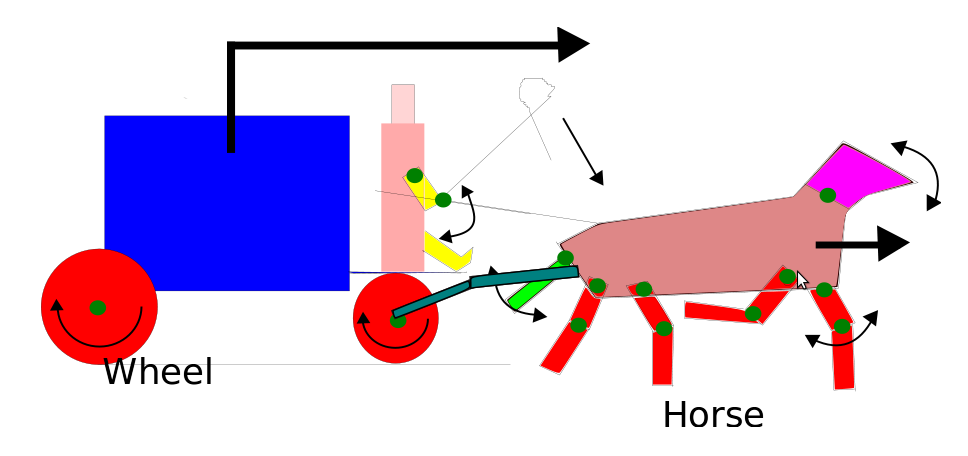
\includegraphics[scale=0.35]{./images/original.png}
	\end{center}
	\subsection*{Brief Description}
	This, horse carriage is our original Project Proposal.It consists of a horse driven cart, and a man steering it. So, it broadly 	consists of 3 parts \\I) The Horse
	\begin{description}
		\item[$\bullet$ ] movable body with degree of freedom along the X-axis
		\item[$\bullet$ ] 2 wheels, with ability to rotate and to travel linearly forward
		\item[$\bullet$ ] rod connecting the carriage to the horse
	\end{description}II) The Man 
	\begin{description}
		\item[$\bullet$ ] Movable hand, holding a whip to start the cart by hitting a horse
	\end{description}
	III) The Horse
	\begin{description}
		\item[$\bullet$ ] Body, this is the main mass of the horse, and moves along with his legs
		\item[$\bullet$ ] 4 legs, the engine of our transport system, moves ahead and also allows rotation in knees
		\item[$\bullet$ ] Tail of the horse, moves at will
		\item[$\bullet$ ] Horse's head, nods 
	\end{description}
	\begin{center}
	\subsubsection*{Final Box2d Simulation}
	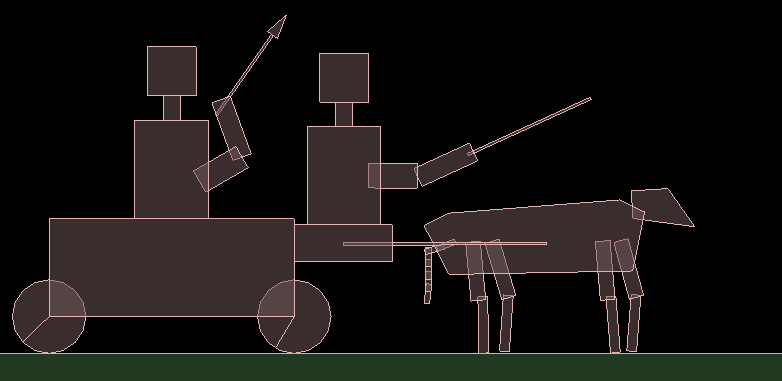
\includegraphics[scale=0.35]{./images/final.png}
	\end{center}
	\subsection*{The Final Project}
		As, can be seen from the pictures above, and the simulation, the project has ticked all the boxes in terms of the initial 			proposal.We have also had time to make an adition to the original design.
		\\I) ADDITIONS : The Warrior
	\begin{description}
		\item[$\bullet$ ] Sits on the chariot, and moves ahead
		\item[$\bullet$ ] Holds a spear in his arm
		\item[$\bullet$ ] Releases the spear in a specified direction when given a keypress
	\end{description}
	
	II) INTERESTING FEATURES
	\begin{description}
		\item[$\bullet$ ] The horses movements have been made continuous and are well synchronised, thanks to changes in step function.
		All stuff about Box2d are referred from \cite{box2d} and \cite{box}.
		\item[$\bullet$ ] The horse's tail is a delight to watch, moves on its own
		\item[$\bullet$ ] Arm movements of both men are very natural
	\end{description}
	\section*{Analysis of Graphs of The Project}
\subsection*{Graph 1: Plot depicting Average Step and Loop times (vs) iteration number}
The loop-time increases as the iteration number increase, and it is not difficult to see why. For every additional loop iteration, more time is consumed. And therefore as the iterations increase, the loop time also increases.
\newline The average steptime, is seen better in Graph 2. \newline {\it x} iterations of the loop, consists of {\it x} distinct steps of our simulation.
Thus the average is the sum of times of all {\it x} steps divided by {\it x}. Since the graph is not a horizontal curve, we can 
easily conclude that all steps of our simulation are not taking the same amount of time.Initially the average step time is decreasing, implying that time taken per step decreases for the initial steps . But after some 800 iterations, the graph starts to rise, meaning that step 800 onwards, each step of the simulation is taking more time.
\newline\newline L=Loop time, i=time taken for ith step, N=Iteration Number and S=average step time
\begin{equation}
L=\displaystyle\sum\limits_{i=1}^N i
\end{equation}
\begin{equation}
S=L/N
\end{equation}
\begin{figure}
\begin{minipage}{.5\textwidth}
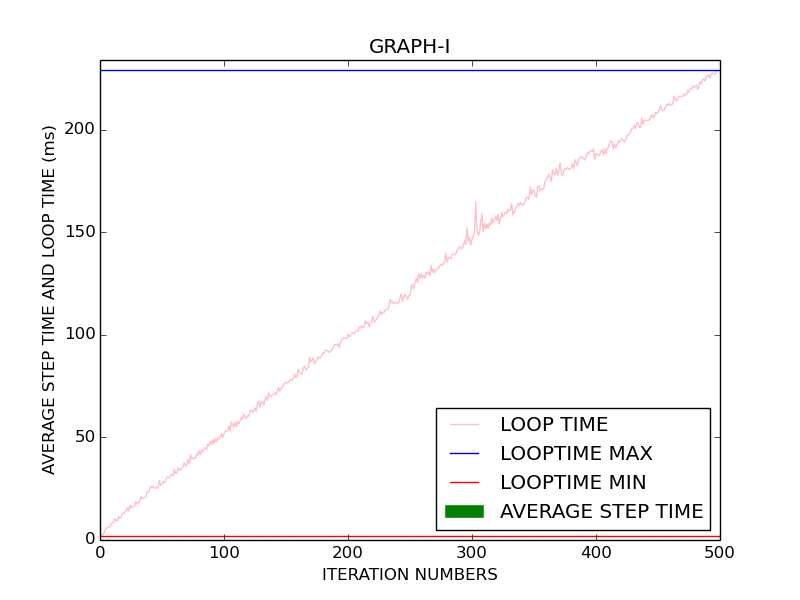
\includegraphics[scale=0.35]{./images/plot1.png}
\caption*{Graph 1}
\end{minipage}
\begin{minipage}{.5\textwidth}
\includegraphics*[scale=0.35]{./images/plot2.png}
\caption{Graph 2}
\end{minipage}
\end{figure}

\subsection*{Graph 2: Plot depicting Average times (vs) iteration number}
The slopes of these average times i.e Average Step (S), Vellocity (V), Collision (C) and Position time(P) are similar to each other.This shows that averge step time includes these individual times, and its behaviour is very much dictated by these individual components of it.\newline
The sum time(X) is
\begin{equation}
X=P+C+V
\end{equation}
\newline
And the time taken by the Velocity is more than that by the Collision and Position iteration calculations. And this is why the Sum curve
and the Velocity curve are adjacent.
\subsection*{Analysing these graphs for a heavy system}
We ran the executable with the system being in a heavily loaded (90 \% )state. As it was taking significantly more time than it took earlier,
we have run only upto 100 iterations.
Actually on carefully monitoring the cpu using {\it top} command we observed  that the EXECUTABLE sometime takes a large chunk of cpu in other time the programs share the space that might explain the large irregularities in the graph.
\begin{figure}
\begin{minipage}{.5\textwidth}
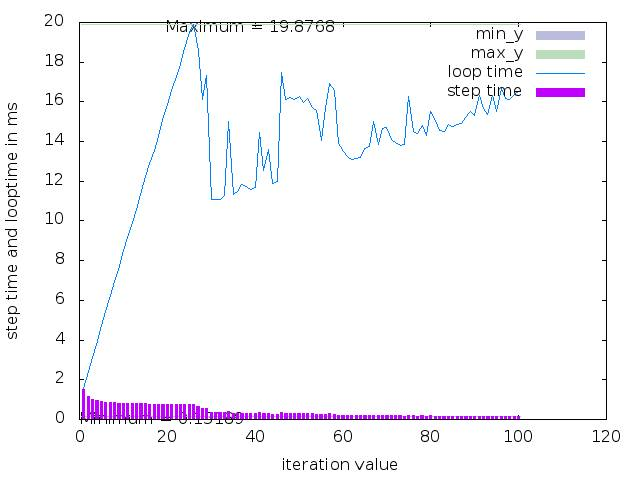
\includegraphics[scale=0.35]{./images/plot1heavy.png}
\caption{Graph 1 heavy}
\end{minipage}
\begin{minipage}{.5\textwidth}
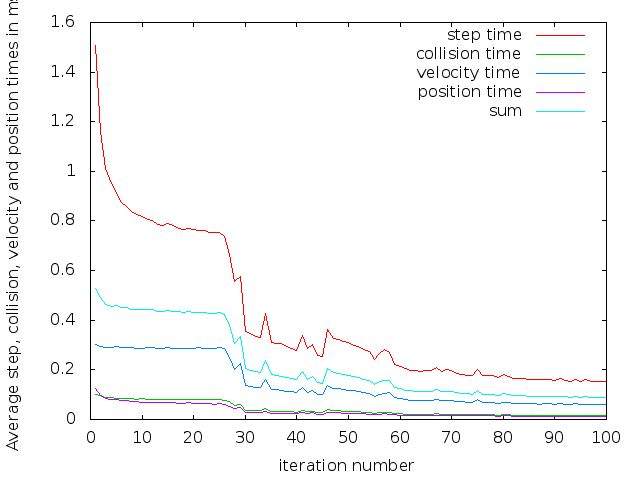
\includegraphics[scale=0.35]{./images/plot2heavy.png}
\caption{Graph 2 heavy}
\end{minipage}
\end{figure}
\subsection*{Graph 3: Plot depicting Average Step Error Bars (vs) iteration number}
When the iteration number is high the input sent to main.cpp being larger, the output is an average over a greater number. Thus the error nullifies when averaged over larger samples, and hence the error output attained at higher iterations is lower. This explains the decreasing error as the no. of iterations increase.
\subsubsection*{Graph 3}
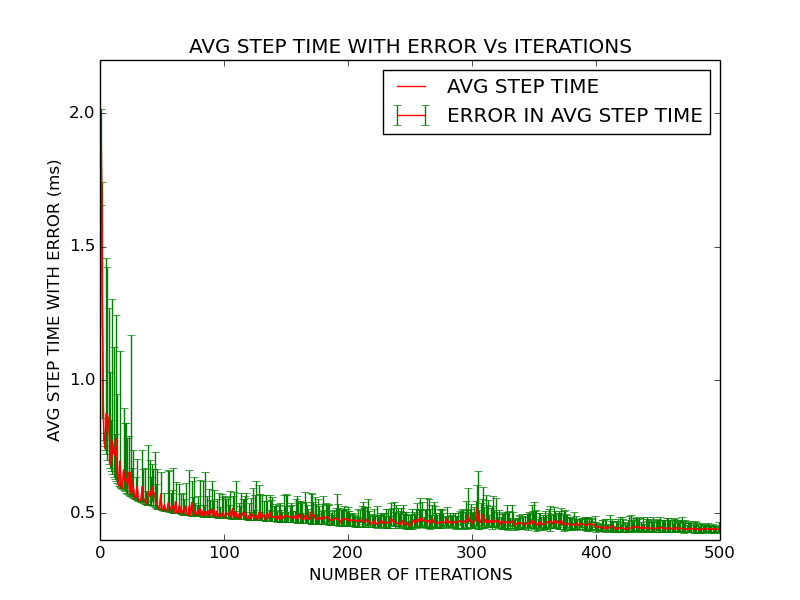
\includegraphics[scale=0.35]{./images/plot3.png}
\subsection*{Graph 4: Depicting The Frequency Plot For Avg Step Time}
Most of the avg step times(for various rerun numbers) lie in the same bucket as the actual avg step time in our Histogram, whereas the points lying outside this bucket may have occured due to {\it experimental errors}.
\subsubsection*{Graph 4}
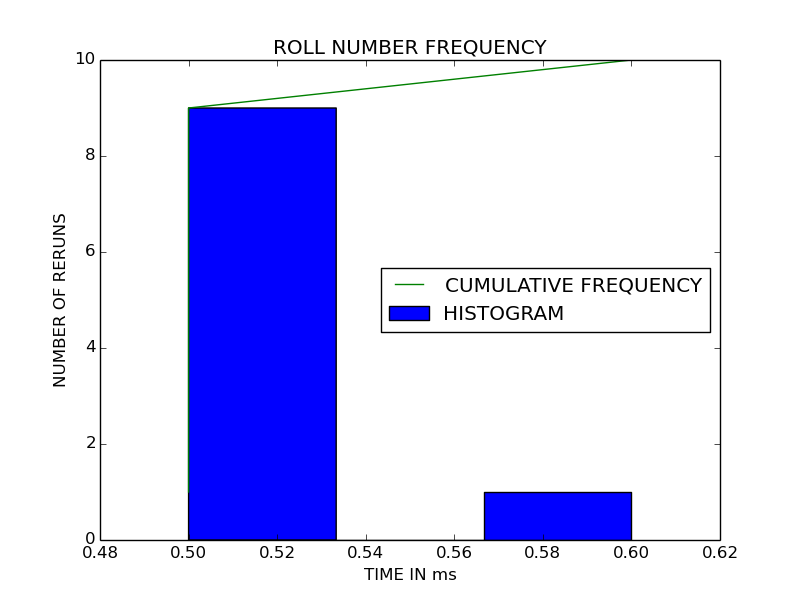
\includegraphics[scale=0.35]{./images/plot4.png}
\subsection*{Graph 5: Comparing Average Step Time of Full Sample and Random Sample}
When the number of iterations are large, it can be observed that the two
graphs converge to a similar function and hence the best fit line is almost the same. This is due to the fact that
when the iterations are huge, the number of data points is large and hence the error converges to zero. On the
other hand, when we took a lower number of iterations, we could see the difference in the best fit lines of the two.
\subsubsection*{Graph 5}
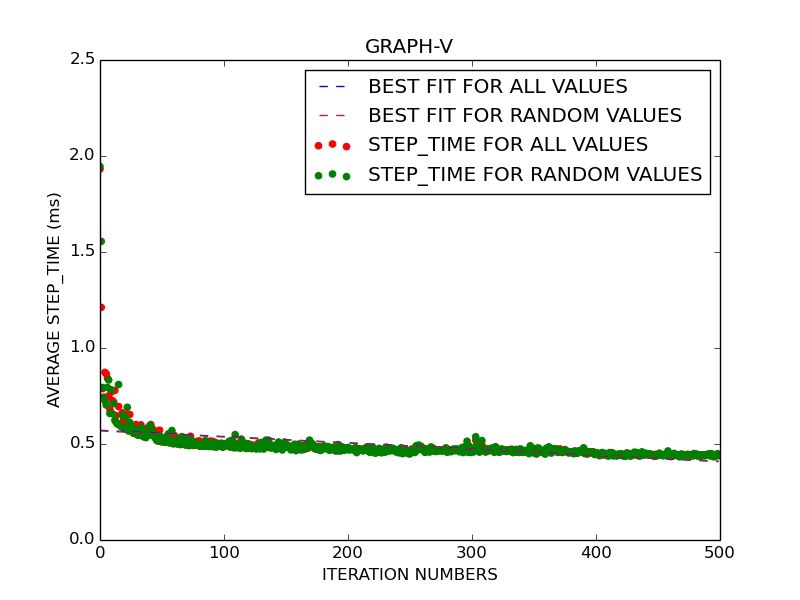
\includegraphics[scale=0.3]{./images/plot5.png}
\subsubsection*{Graph 5 for smaller data}
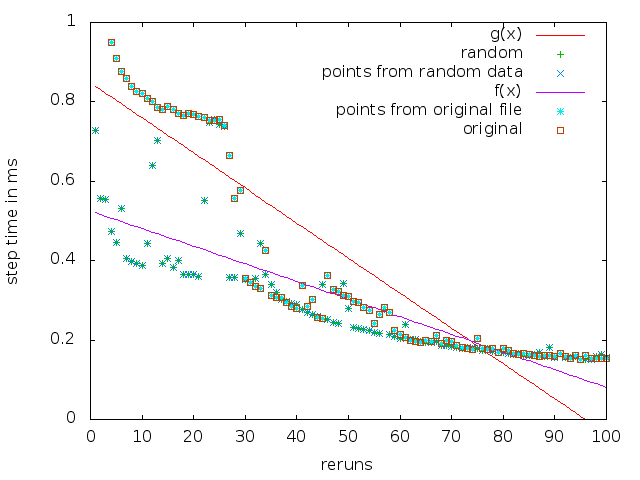
\includegraphics[scale=0.25]{./images/g16_plot5.png}
\section*{Understanding the time and gettimeofday() }
The time command, gives us three separate times - real,user and sys. The real time gives us the total time passed, when a particular operation is being run along with the time command. The user time, gives us the time required by that particular opertion and does not include the times of other applications that might be running along with the timed operation. In cases where the computer is not loaded with other operations, these two are fairly the same, although for obvious reasons real time is slightly more than user time. sys time gives us the time the operation spends in interacting with the memory and other components of the OS.\newline The gettimeofday function gives the current time, and hence difference between two gettimeofday functions, at the begining and end of the operation shall work similar to the real time of the time command.

\section*{Analysing difference between the two cmake commands Debug Mode and Release Mode}

\begin{description}
\item[$\bullet$ ] On running the executable for 100000 iterations, in both the Modes, it is quite easy to see that the loop time required for the 
Debug Mode (95.92 s)
 is more than that of the Release Mode (9.38 s) with -O3 flags. We have observed the .dat files of the two to get more details.
\newline
\item[$\bullet$ ]
 Compared to the debug data, the release data has skipped quite a few functions. Also, the number of calls made to each function,
   is far less in the release mode than in the debug mode,as a result of optimization flags. One also sees, that each function 
   takes more
   time in debug mode than in release mode. For example the function {\bf b2Vec2::b2Vec2(float, float)} takes 0.31 s in the 
   release mode and 2.31s in debug mode.Operator functions also take one-tenth of the time in release mode of what they take in 
   debug mode.
\newline
\item[$\bullet$ ]
The operator functions on the b2Vec2 variables also take a humungous amount of time in the debug mode compared to the release mode, where they take no noticable time.This is because the debug mode considers only pure functions.
   \newline 
\item[$\bullet$ ]
Several functions that are not even called in the release mode, take around 2s of the time in the debug mode.
   \newline 
\item[$\bullet$ ]
The -On flags also play a very important role.In absence of optimization 
   option, compiler tries to decrease the cost of compilation. When we enable those flags (eg. -O2 -O3), compiler optimizes the 
   performance at a cost of compilation time.\newline
\item[$\bullet$ ]
In release mode, we enable -O3 flags and it tries to do optimization. Optimizations can greatly complicate debugging and hence it takes
 more time while compiling.But When we run it for 100000 iterations, the cumilative time is only 3.11s. For debug mode, we remove -On flags. Now, the compiler wants to decrease the cost of compilation and to make debugging produce the expected results. It does not optimize the binary it produces. Hence, it takes relatively less time for compiling. But for same number of iterations, cumilative time comes out to be 59.98s (much larger than 6.37s). 
\newline
\item[$\bullet$ ]
The method, b2RevoluteJoint::SolveVelocityConstraints(b2SolverData const\&), takes maximum time in both the modes, 12.72 \% (0.81 s)in release mode and 4.17 \% in debug mode (2.50 s) . 
\newline
\item[$\bullet$ ]
Lot of the time is also taken by revolute joints, and is more or less unavoidable.Although fixtureDef were made as generic as possible to reduce over use.
\newline
\item[$\bullet$ ]
Use of b2Vec2 and other velocity constraints is again very important from the logic point of our code. Hence optimising the Box2d part for these time intensive functions can be done.
\newline
\item[$\bullet$ ]
In a previous version of the code, we also noticed that since we were running the set angle for a lot of iterations, while making the hand movement, we were utilising more than double the time we are geting currently. As a result, we were not only successful in getting a better graphics but also successful in OPTIMISATION.
\newline

These data have been generated using scripts of previous labs \cite{pyscript}
\end{description}

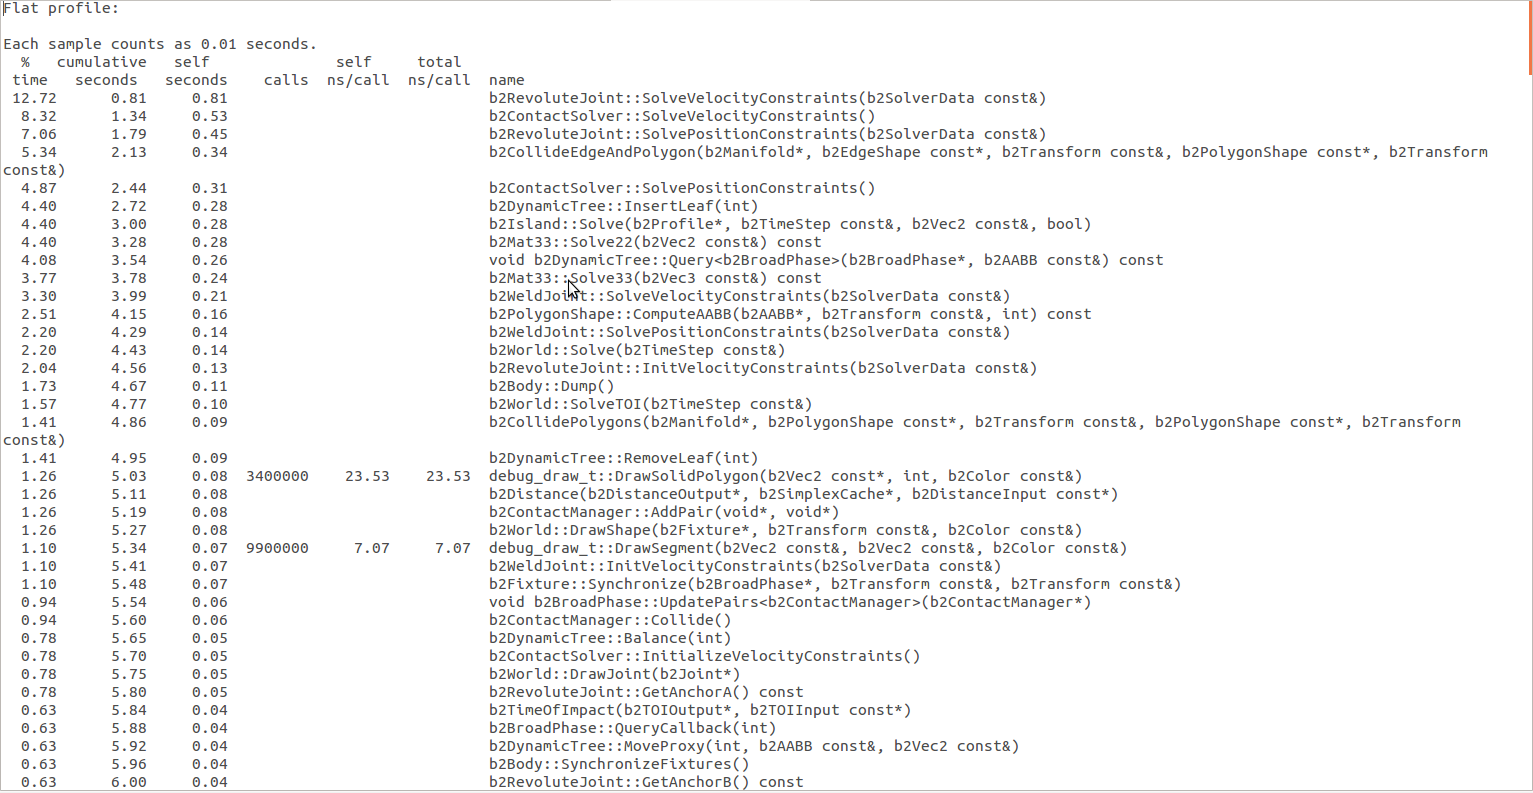
\includegraphics[height=7cm]{./images/debug_dat1.png}

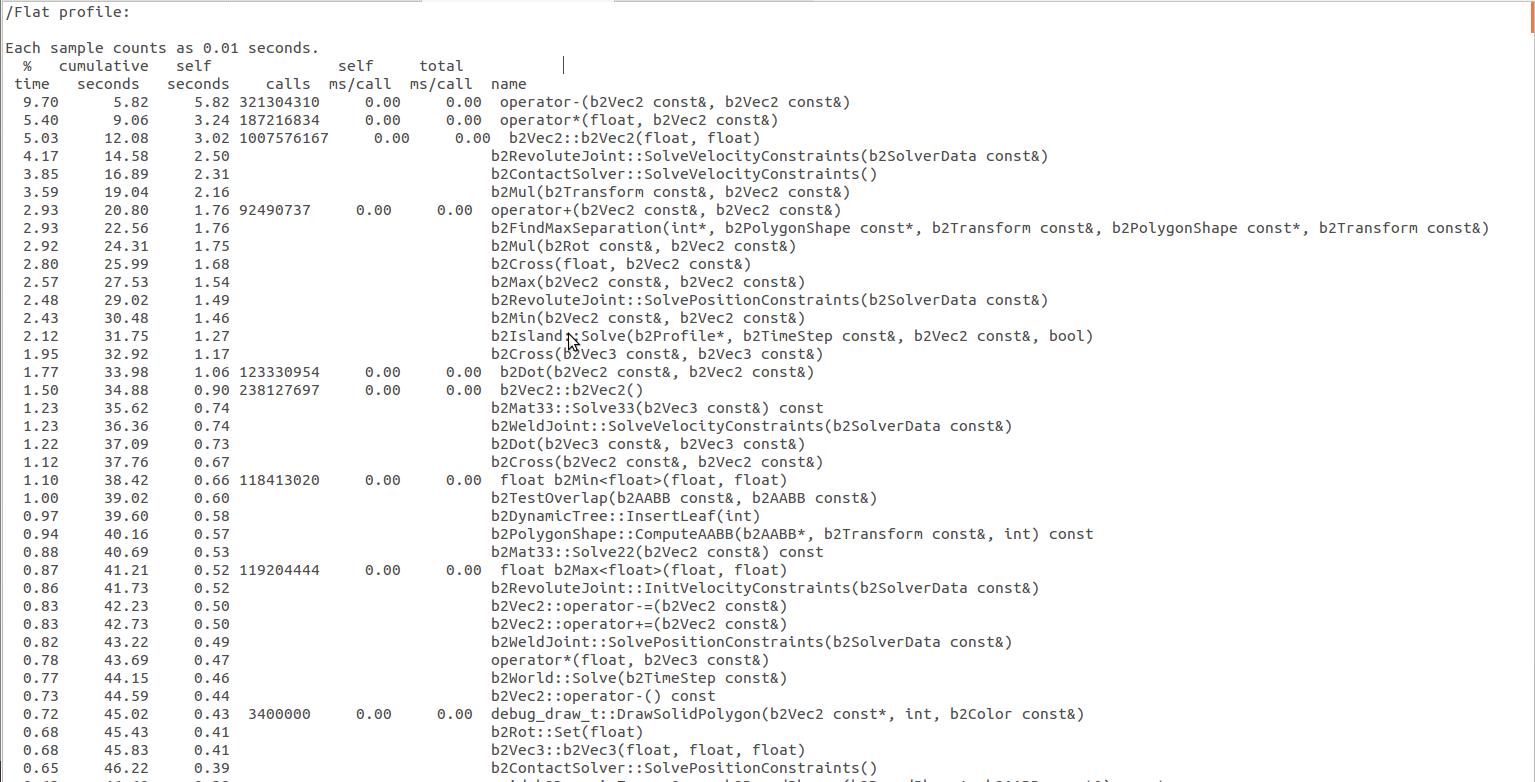
\includegraphics[height=7cm]{./images/release_dat1.png}


\section*{Inference from The Call-Graphs}
\begin{description}
\item[$\bullet$ ]
The call graphs give an extremely crisp and easy to understand depiction of the code. Like any graph, it consists of nodes N - which is a particular function and edges E between two nodes (N1,N2). 
\newline
\item[$\bullet$ ]
It is a directed graph. This is because an edge (N1,N2), will show the calling of the function N2 inside of N1. Each Node also stores, along with its function name, the total fraction of the total time consumed by that function in \%, and in brackets the self time i.e., the time the functions spends after removing the time spent via calls to other children function. It also stores the number of times that that function has been called.The edges between (N1,N2) stores the amount of time taken by the function N2, when N1 calls it. It also shows the number of times N1 calls N2.\newline
\item[$\bullet$ ]
The call graphs of the two Modes, clearly show why there is such a massive difference in times, when both are run. The debug mode has a lot more functions that are called, and call other functions. In case of release mode,this is relatively less.Also, a lot of functions are not even called here. The self times of the functions, are almost the same as the function times in the release mode. But in the debug mode, the self time is significantly less the total time.This shows the difference in the optimization and hence the time difference that results.
\newline
\item[$\bullet$ ]
Other important use of callgraphs is the color of a node.The color of node gives us the proportionality of time directly so if we want to optimize some function just cheking the legend could be of great help
\end{description}
\subsection*{Release Mode}

\subsubsection*{Release mode enlarged}
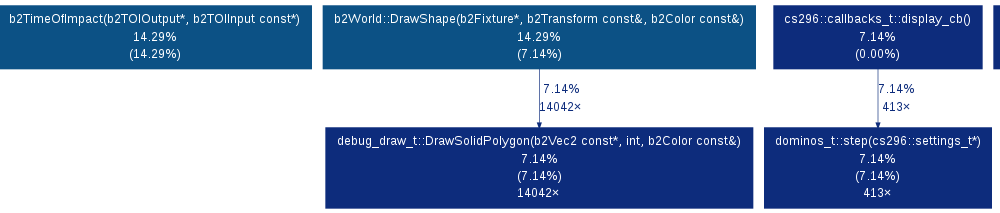
\includegraphics[scale=0.30]{./images/rcall1.png}
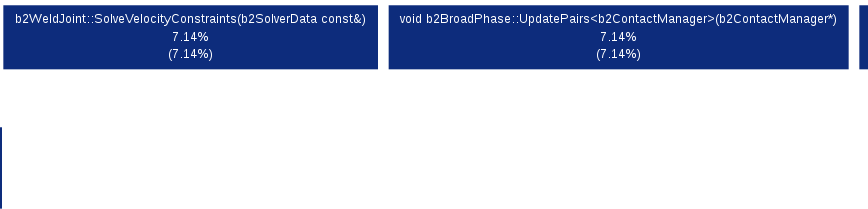
\includegraphics[scale=0.30]{./images/rcall2.png}
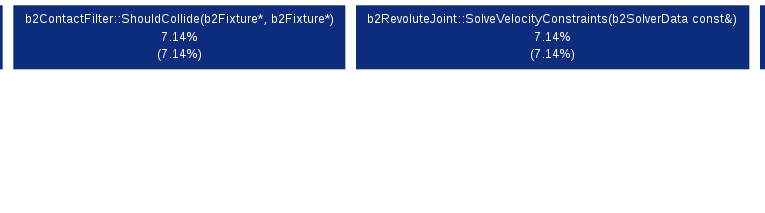
\includegraphics[scale=0.30]{./images/rcall3.png}
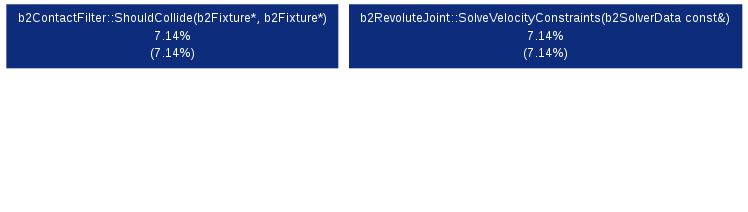
\includegraphics[scale=0.30]{./images/rcall4.png}
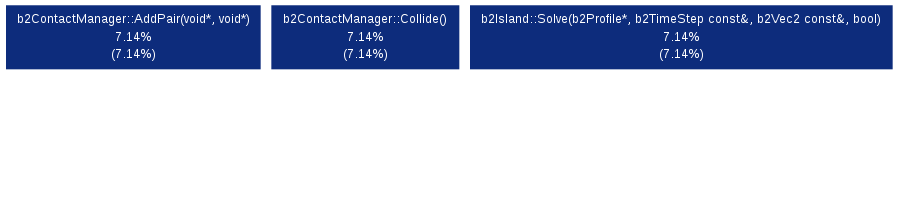
\includegraphics[scale=0.30]{./images/rcall5.png}
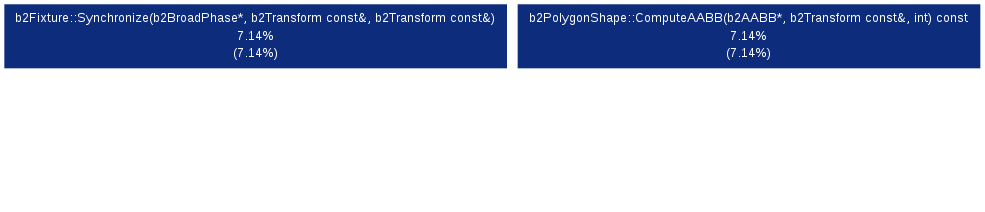
\includegraphics[scale=0.30]{./images/rcall6.png}
\subsection*{Debug Mode}

\subsubsection*{Debug mode enlarged}
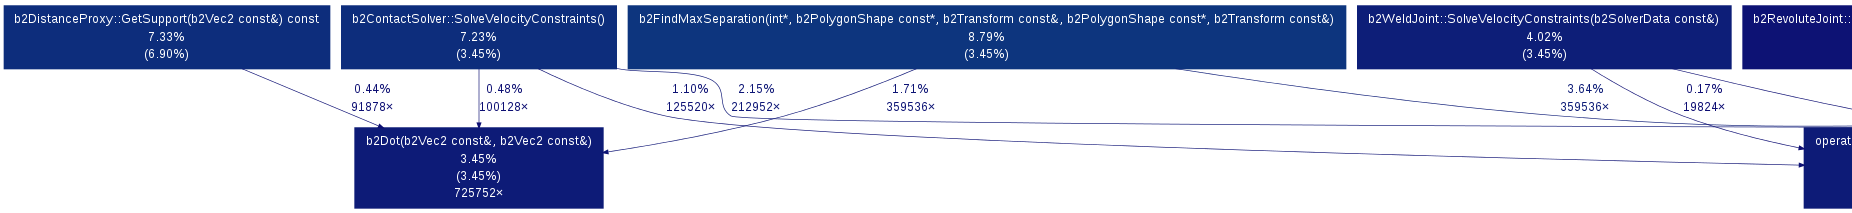
\includegraphics[scale=0.30]{./images/dcall1.png}
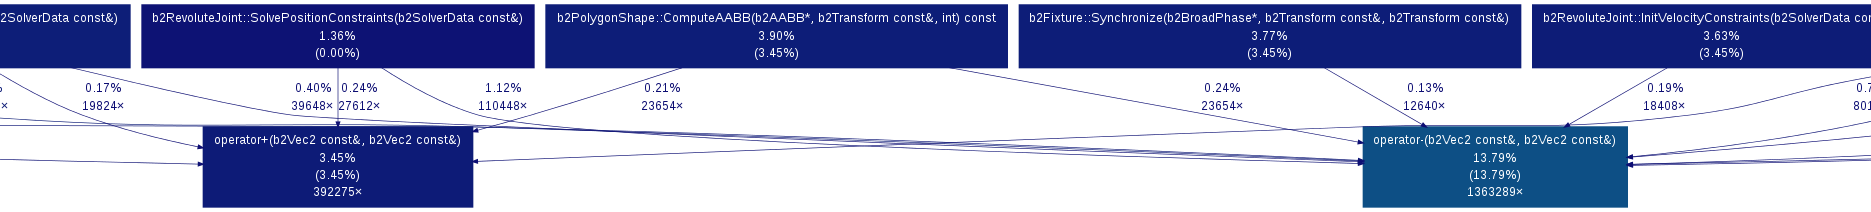
\includegraphics[scale=0.30]{./images/dcall2.png}
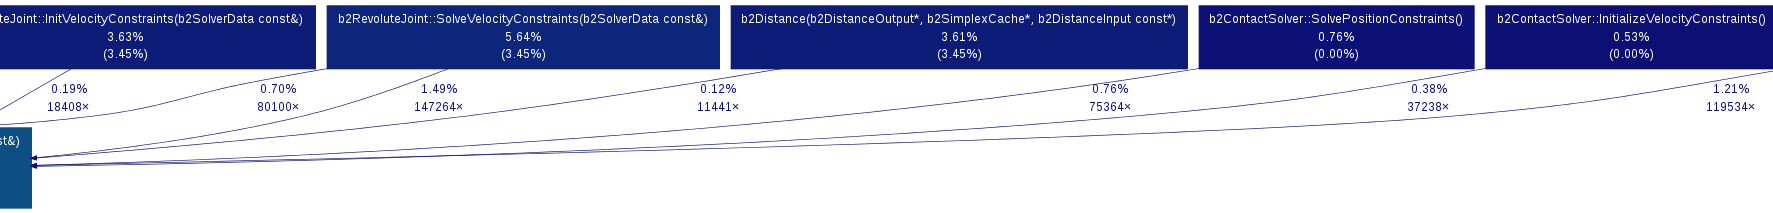
\includegraphics[scale=0.30]{./images/dcall3.png}
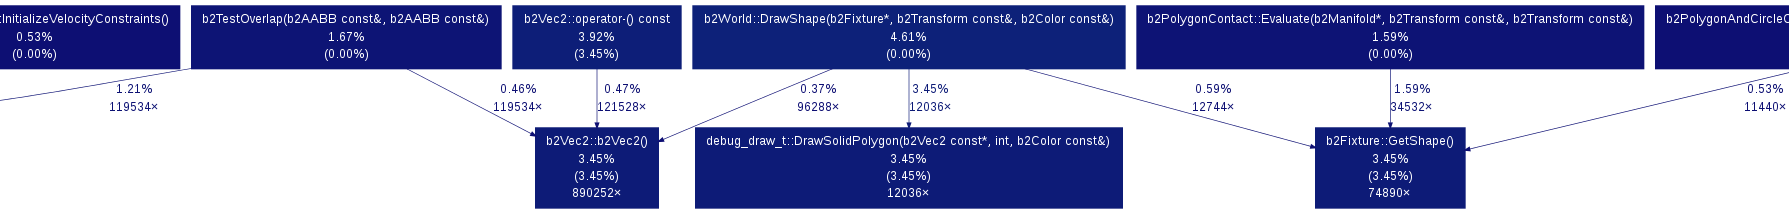
\includegraphics[scale=0.30]{./images/dcall4.png}
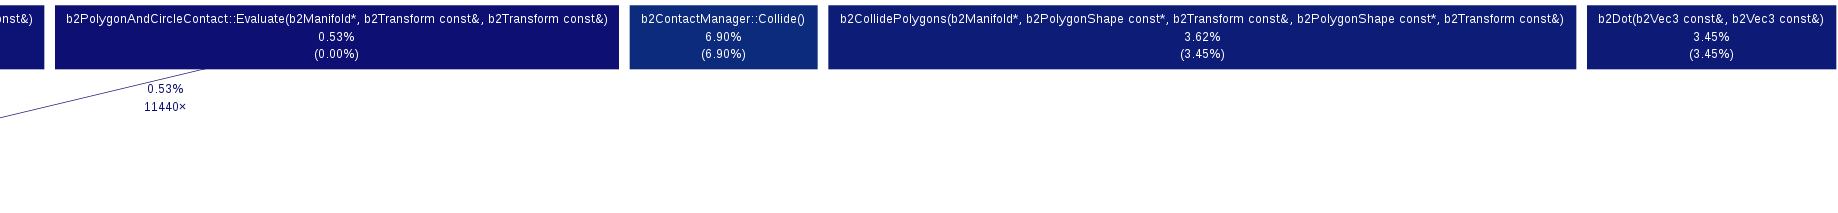
\includegraphics[scale=0.30]{./images/dcall5.png}
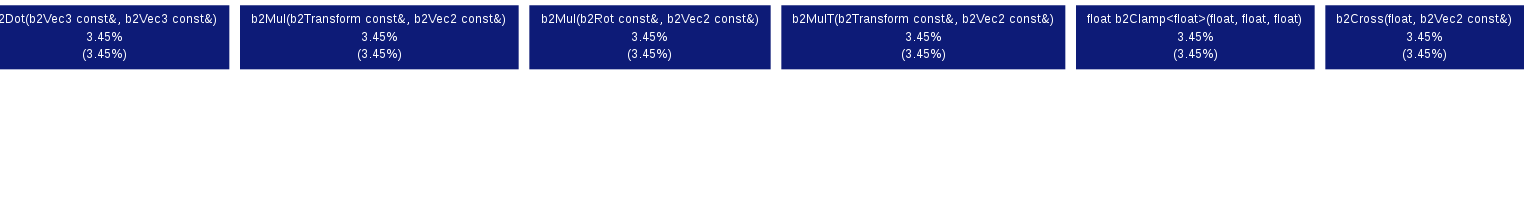
\includegraphics[scale=0.30]{./images/dcall6.png}


\bibliographystyle{plain}
\bibliography{cs296_project_report}
\end{document}
